\documentclass[12pt, a4paper]{report}
\usepackage{style}


\title{Software Engineering II\\ \textit{Exercises}}
\author{Christian Rossi}
\date{Academic Year 2023-2024}

\begin{document}

\maketitle

\newpage

\begin{abstract}
    The objective of the course is to teach the principals methods and processes of software engineering needed to develop complex and qualitative software.
     
    The course covers the following arguments:
    \begin{itemize}
        \item Software process and its organization.
        \item Modelling languages.
        \item Requirements analysis and definition.
        \item Software development methods and tools.
        \item Approaches for verify and validate the software.
    \end{itemize}
\end{abstract}

\cleardoublepage
\pagenumbering{Roman}

\tableofcontents

\cleardoublepage
\pagenumbering{arabic}

\chapter{Exercises session I}
    \section{AdmissionManager}
        Your company has been tasked to develop a system that handles the admission applications that parents send, on behalf of their children, to the high schools of a metropolitan
        area. Parents can send admission applications to multiple schools. Before sending an application, they must register their child in the system; the registration includes 
        login credentials (username and password), the personal data of the child (first name, last name, birthdate, etc.), the name of at least one parent, contact information 
        (which must include an email address and a phone number), the name of the last school they attended, and the list of grades (which includes the obtained score, from 1 to 10, 
        for each subject). Each application is assigned an identifier by the system, to allow parents to check its status after sending it (which can be “accepted”, “rejected”, or 
        “not evaluated”). Parents can withdraw applications previously sent. They can also ask the system to be notified by email when the outcome of the evaluation of an application
        is available. School administrators use the system to check the applications sent to their schools and to approve/reject them. In particular, they can retrieve the list of 
        applications sent to their schools that have yet to be evaluated; they can also leave comments on the applications, and they can decide to accept or reject the applications.
        Administrators can also set a preference to receive a notification, in the form of an email, when a new application is sent to their school.
        \begin{enumerate}
            \item Define the goals for the AdmissionManager system.
            \item Select one of the goals defined in the previous point and define in natural language suitable domain assumptions and requirements to guarantee that the 
                AdmissionManager system fulfills the selected goal.
            \item Draw a UML Use Case Diagram describing the main use cases of the AdmissionManager system.
            \item Pick one of the use cases, and define it. 
        \end{enumerate}
    \subsection*{Solution}
        \begin{enumerate}
            \item The goals are world phenomena shared between the machine and the real world. They are problem of the real world that the AdmissionManager needs to address. We have 
                four examples, which are: 
                \begin{itemize}
                    \item User sends an application.
                    \item User withdraws an application.
                    \item School administrator evaluates an application.
                    \item User is notified about an application evaluation. 
                \end{itemize}
                The problem with those goals is that they are only on world side, so they are not well formulated. The term user is ambiguous, it needs to be specified (parents and school 
                administrator). The formulation can be changed to make them correct: 
                \begin{itemize}
                    \item Parents can manage (send and then monitor) applications to schools on behalf of their children.
                    \item School administrators can manage (check and approve/reject) applications sent to their schools.
                \end{itemize}
            \item A domain assumption like "as soon as an application arrives to the system, a status needs to be assigned to it" is not correct because the status depend on a method in 
                the program and not on something that is granted by the real world. Examples of correct domain assumption, that are not well formulated are: 
                \begin{itemize}
                    \item Parents must be registered into the system to issue an application. 
                    \item The system must allow parents to register by providing their email address and personal information.  
                \end{itemize}
                In the end, for the first goal we have the following domain assumptions: 
                \begin{itemize}
                    \item AdmissionManager allows system administrators to open application windows for their schools.
                    \item AdmissionManager allows parents to register into the system and provide contact information and information about their child. 
                    \item AdmissionManager allows parents to log into the system using the credentials input at registration time.
                    \item AdmissionManager allows parents to indicate in their profile that they want to be notified when the outcome of an application is available. 
                    \item AdmissionManager allows parents to send an application to a school. 
                    \item AdmissionManager assigns a unique identifier to each application received. 
                    \item AdmissionManager allows parents to see the list of applications sent.
                    \item AdmissionManager allows parents to withdraw an application previously sent.
                \end{itemize}
                The assumption is the following: 
                \begin{itemize}
                    \item Parents provide correct information (in particular, contact information) when registering.
                \end{itemize}

                And for the second goal we have the following domain assumptions: 
                \begin{itemize}
                    \item AdmissionManager allows system administrators to insert new administrators in the system and associate them with the corresponding school.
                    \item AdmissionManager allows school administrators to log into the system using the credentials assigned to them by system administrators.
                    \item AdmissionManager allows school administrators to indicate in their profile that they want to be notified when new applications for their schools are received.
                    \item AdmissionManager allows school administrators to retrieve applications (related to their schools) that have yet to be evaluated.
                    \item AdmissionManager allows school administrators to select an application yet to be evaluated and leave a comment in it. 
                    \item AdmissionManager allows school administrators to accept/reject an application. 
                \end{itemize}
                The assumption is the following: 
                \begin{itemize}
                    \item School administrators periodically evaluate applications and guarantee to explicitly accept/reject all applications arrived within the notification window.
                \end{itemize}
            \item The UML use case diagram is the following: 
                \begin{figure}[H]
                    \centering
                    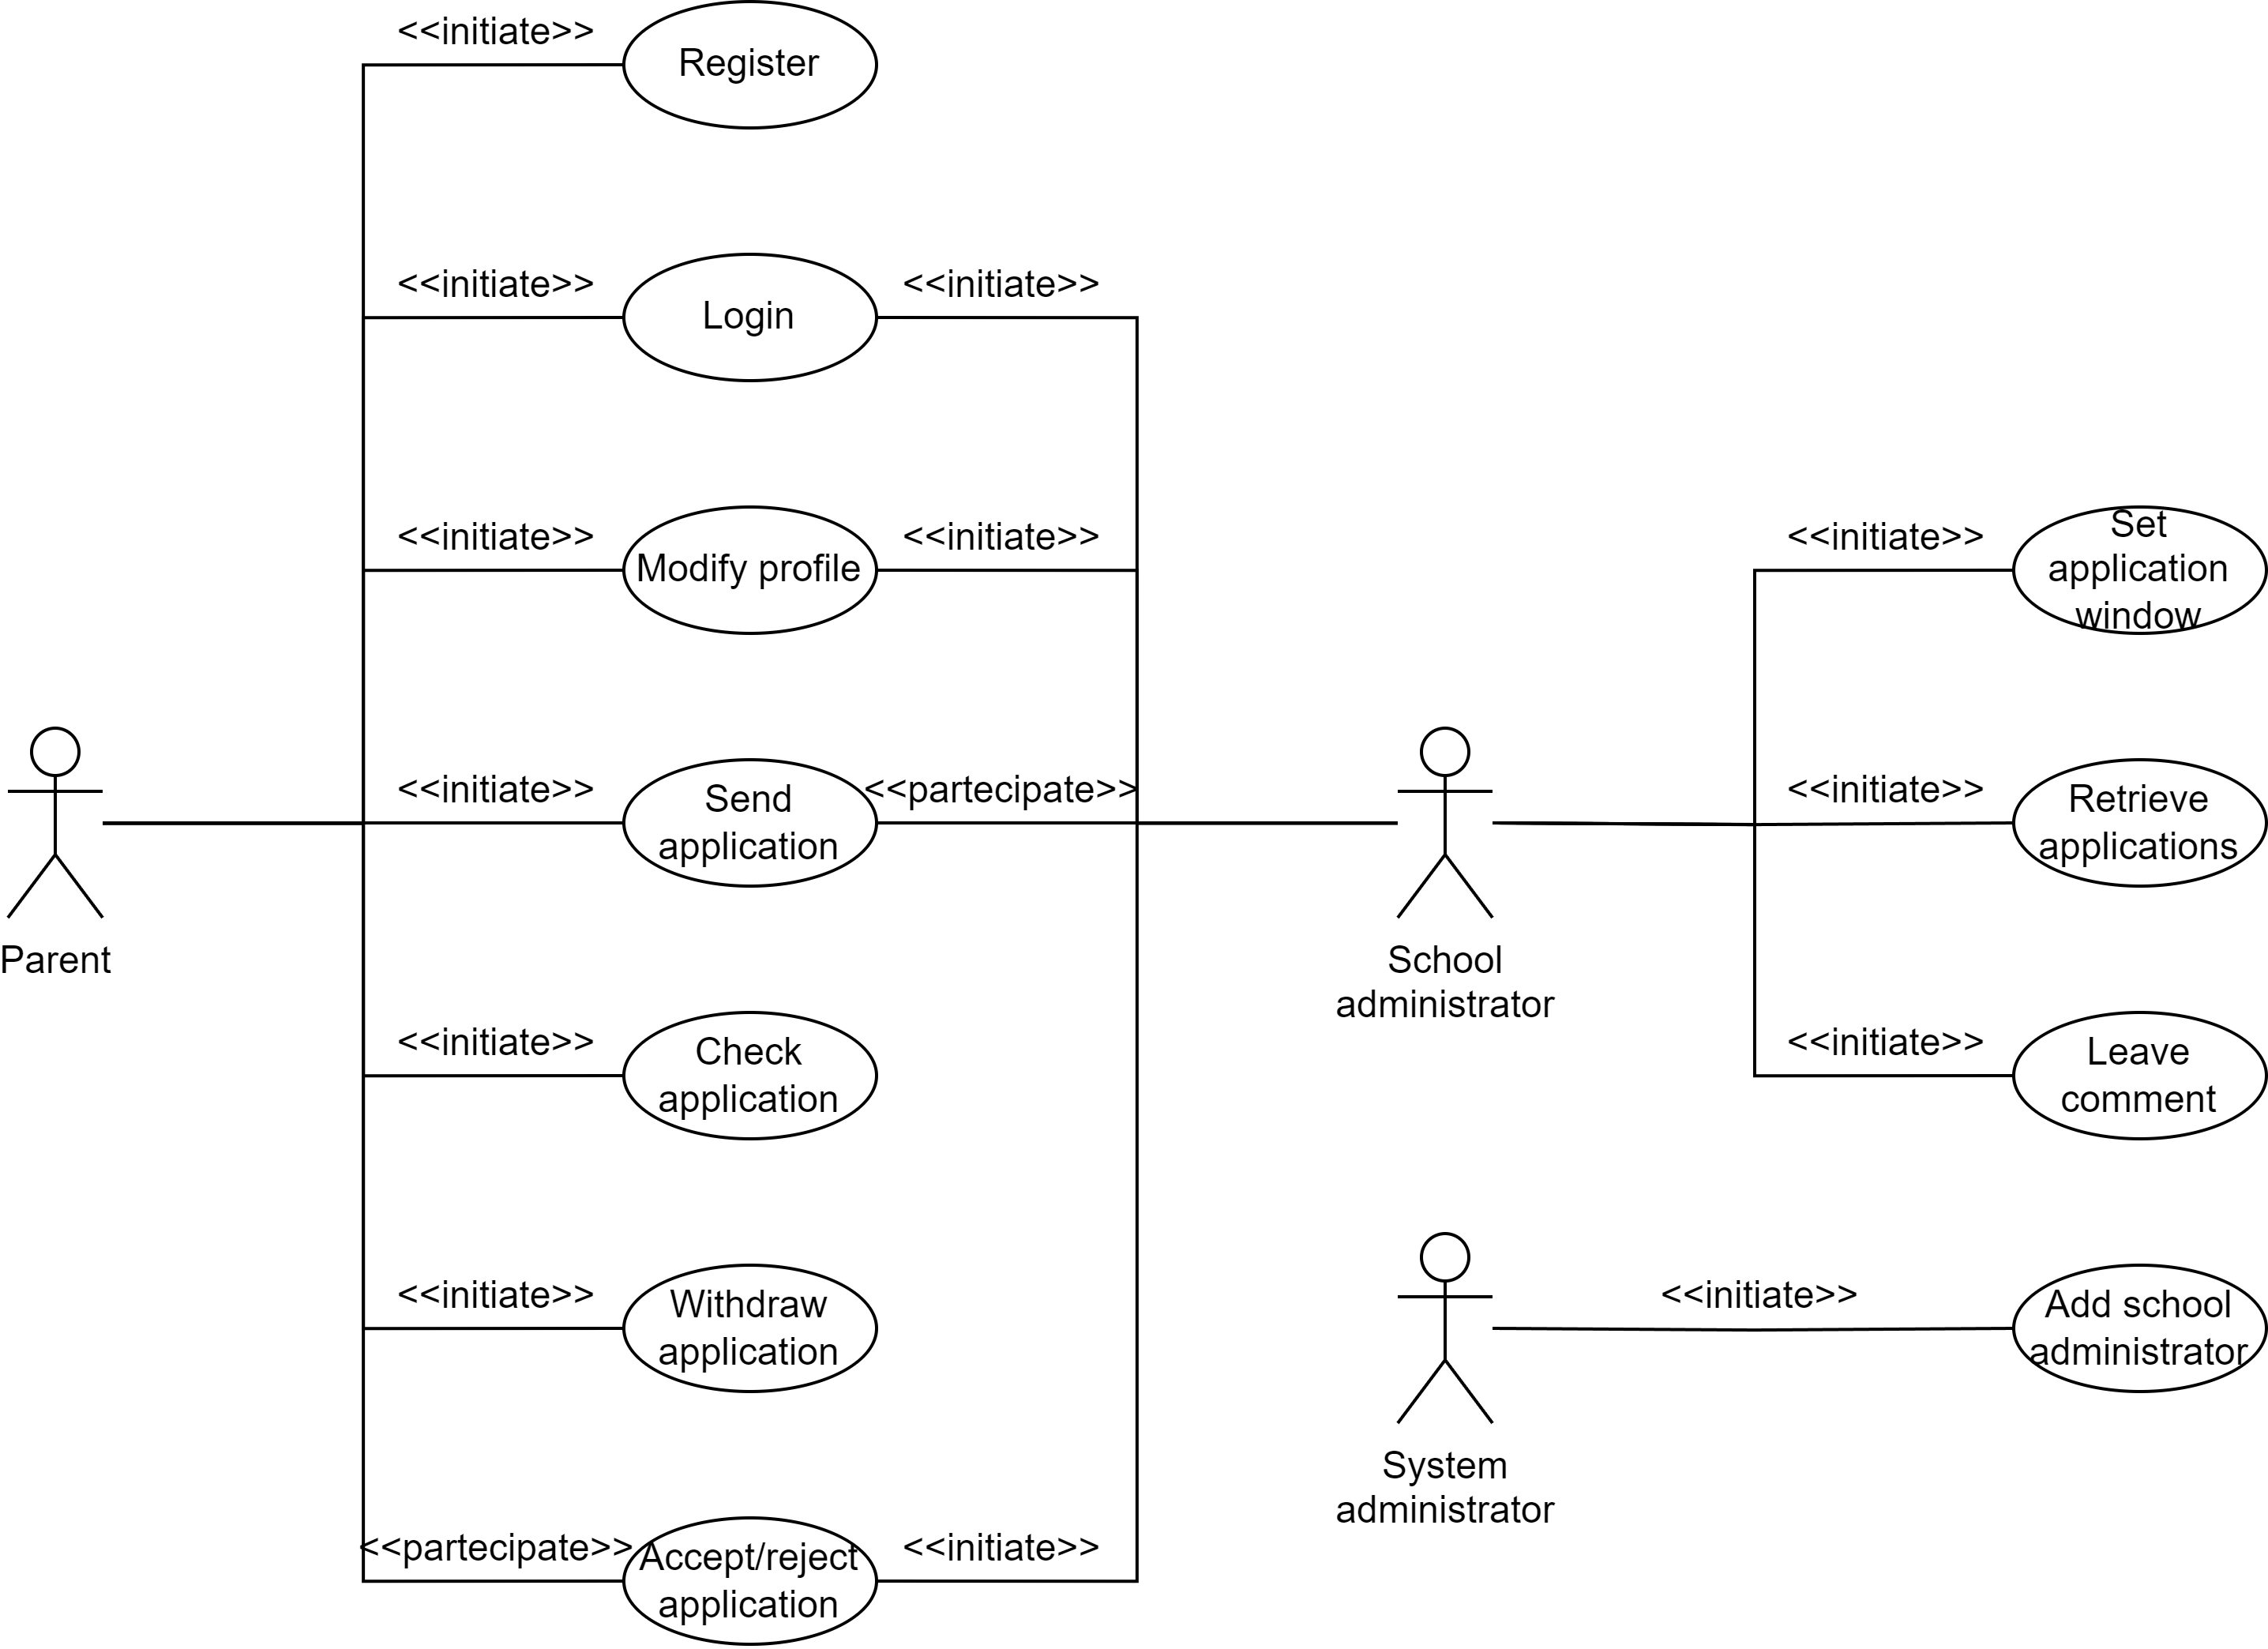
\includegraphics[width=1\linewidth]{images/usecase.png}
                \end{figure}
            \item We select send application case. We have that: 
                \begin{figure}[H]
                    \centering
                    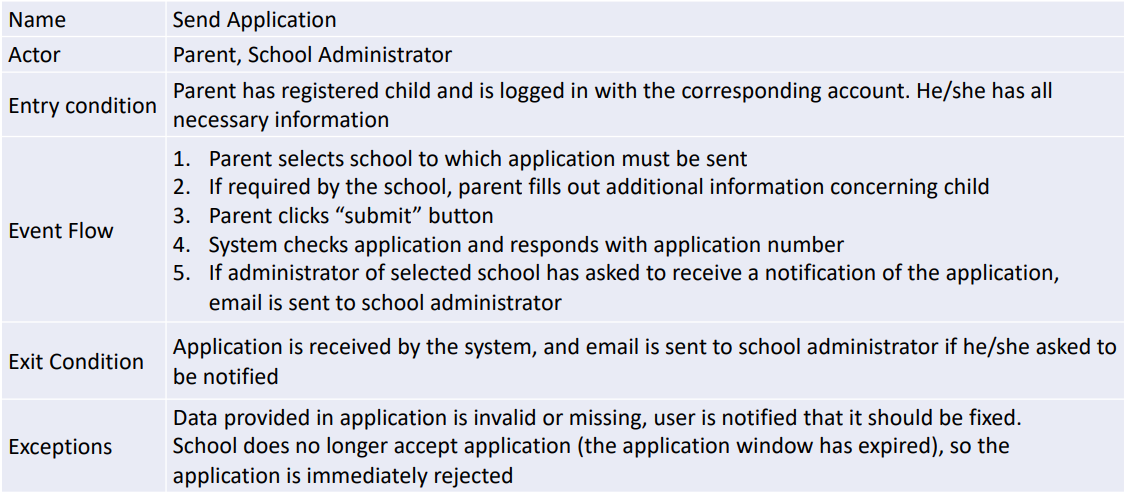
\includegraphics[width=0.9\linewidth]{images/sendapplication.png}
                \end{figure}
        \end{enumerate}

    \newpage

    \section{PaasPopCoin}
        The private security and event organization company HSG from the Netherlands wants to build an application (PaasPopCoin) that handles the coin emission and transactions in 
        the scope of a medium-size music festival they are organizing. The goal of the system is to allow festival-goers and operators to spend an allotted amount of money in 
        relative safety and without the need to bring wallets and other assets around the event. The software in question needs to handle at least three scenarios:
        \begin{itemize}
            \item Emission of coins in exchange for money through appropriate cashier desks and ATMs.
            \item Cash-back, that is, exchange of coins with cash in the same locations (we assume that people at the festival may be willing to receive back the money corresponding
                to the coins they have not used).
            \item Tracking of coin expenditure transactions at the various festival shops.
        \end{itemize}
        In the scope of the above scenarios, there are several special conditions to be considered. First, in the scope of coin emissions, there exist four classes of coin buyers: 
        \begin{itemize}
            \item [a.] VIPs who receive a $30\%$ discount on the coins they buy. 
            \item [b.] Event organization people who receive a $50\%$ discount. 
            \item [c.] Event ticket holders class A, who receive a $20\%$ discount. 
            \item [d.] Regular ticket holders who receive no discount.
        \end{itemize}
        When buying coins, users first need to authenticate themselves by inserting their own ID card in the ATM or by giving it to the cashier; this allows the system to determine 
        the class to which each coin buyer belongs. After authentication, buyers get the coins upon inserting into the ATM or giving to the cashier the corresponding amount of money.
        Second, also in the context of cash-back, users need to authenticate with their ID card to make sure the appropriate amount of money is given back, considering their role and 
        privileges. Third, during the event, every shop clerk keeps track through the PaasPopCoin system of the sales of products and the coins received. PaasPopCoin relies on a 
        third-party analytics service to periodically check whether the festival is earning money or not (cost-benefit analysis). Such check is performed with respect to costs of 
        products being sold during the event, as well as the overhead to cover all event organization and management expenses. 
        \begin{enumerate}
            \item With reference to the Jackson-Zave distinction between the world and the machine, identify the relevant world phenomena for PaasPopCoin, including the ones shared 
                with the machine, providing a short description if necessary. For shared phenomena specify whether they are controlled by the world or the machine. Focus on phenomena 
                that are relevant to describe the requirements of the system.
            \item Describe through a UML Class Diagram the main elements of the PaasPopCoin domain. 
            \item Define a UML Use Case Diagram describing the relevant actors and use cases for PaasPopCoin. You can provide a brief explanation of the Use Case Diagram, especially 
                if the names of the use cases are not self-explanatory.
        \end{enumerate}
    \subsection*{Solution}
        \begin{enumerate}
            \item The world-only phenomena can be: 
                \begin{itemize}
                    \item User buys Class A ticket.
                    \item User buys regular ticket.
                    \item VIP is contracted for event.
                    \item Event organization is started and contractors registered.
                    \item Event starts.
                    \item User gives money to cashier (to be converted in coins).
                    \item User gives coins to cashier (to be converted in money).
                    \item User gives ID card to cashier.
                    \item User buys some product at festival.
                    \item The external analytics service checks the success of an event.
                \end{itemize}

                The shared phenomena can be the following: 
                \begin{itemize}
                    \item User inserts money into an ATM machine.
                    \item ID Card is inserted into ATM.
                    \item User inserts coins into an ATM.
                    \item Cashier inserts in the system an ID card number.
                    \item Cashier inserts in the system the amount of money handed by a certain user.
                    \item Cashier inserts in the system the amount of coins returned by a certain user.
                    \item Store clerk inputs in system the amount of coins spent by user in shop.
                    \item The system enables coin emission after checking ID card and inserted amount of money.
                    \item The system enables cash-back after checking ID card and inserted number of coins.
                    \item The system sends data about purchases to the external analytics service.
                \end{itemize}
            \item The UML diagram of the given problem is: 
                \begin{figure}[H]
                    \centering
                    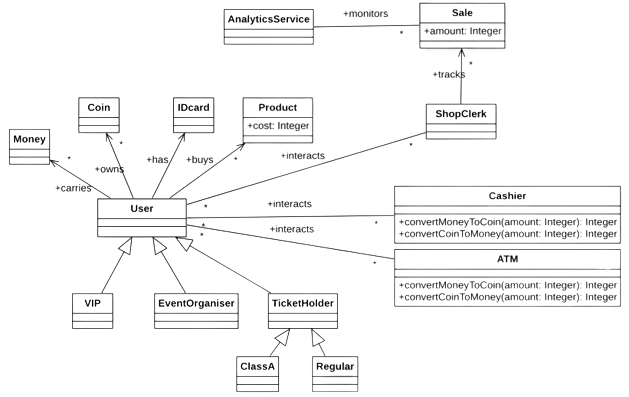
\includegraphics[width=0.9\linewidth]{images/UML.png}
                \end{figure}
            \item The UML use case diagram of the given problem is: 
                \begin{figure}[H]
                    \centering
                    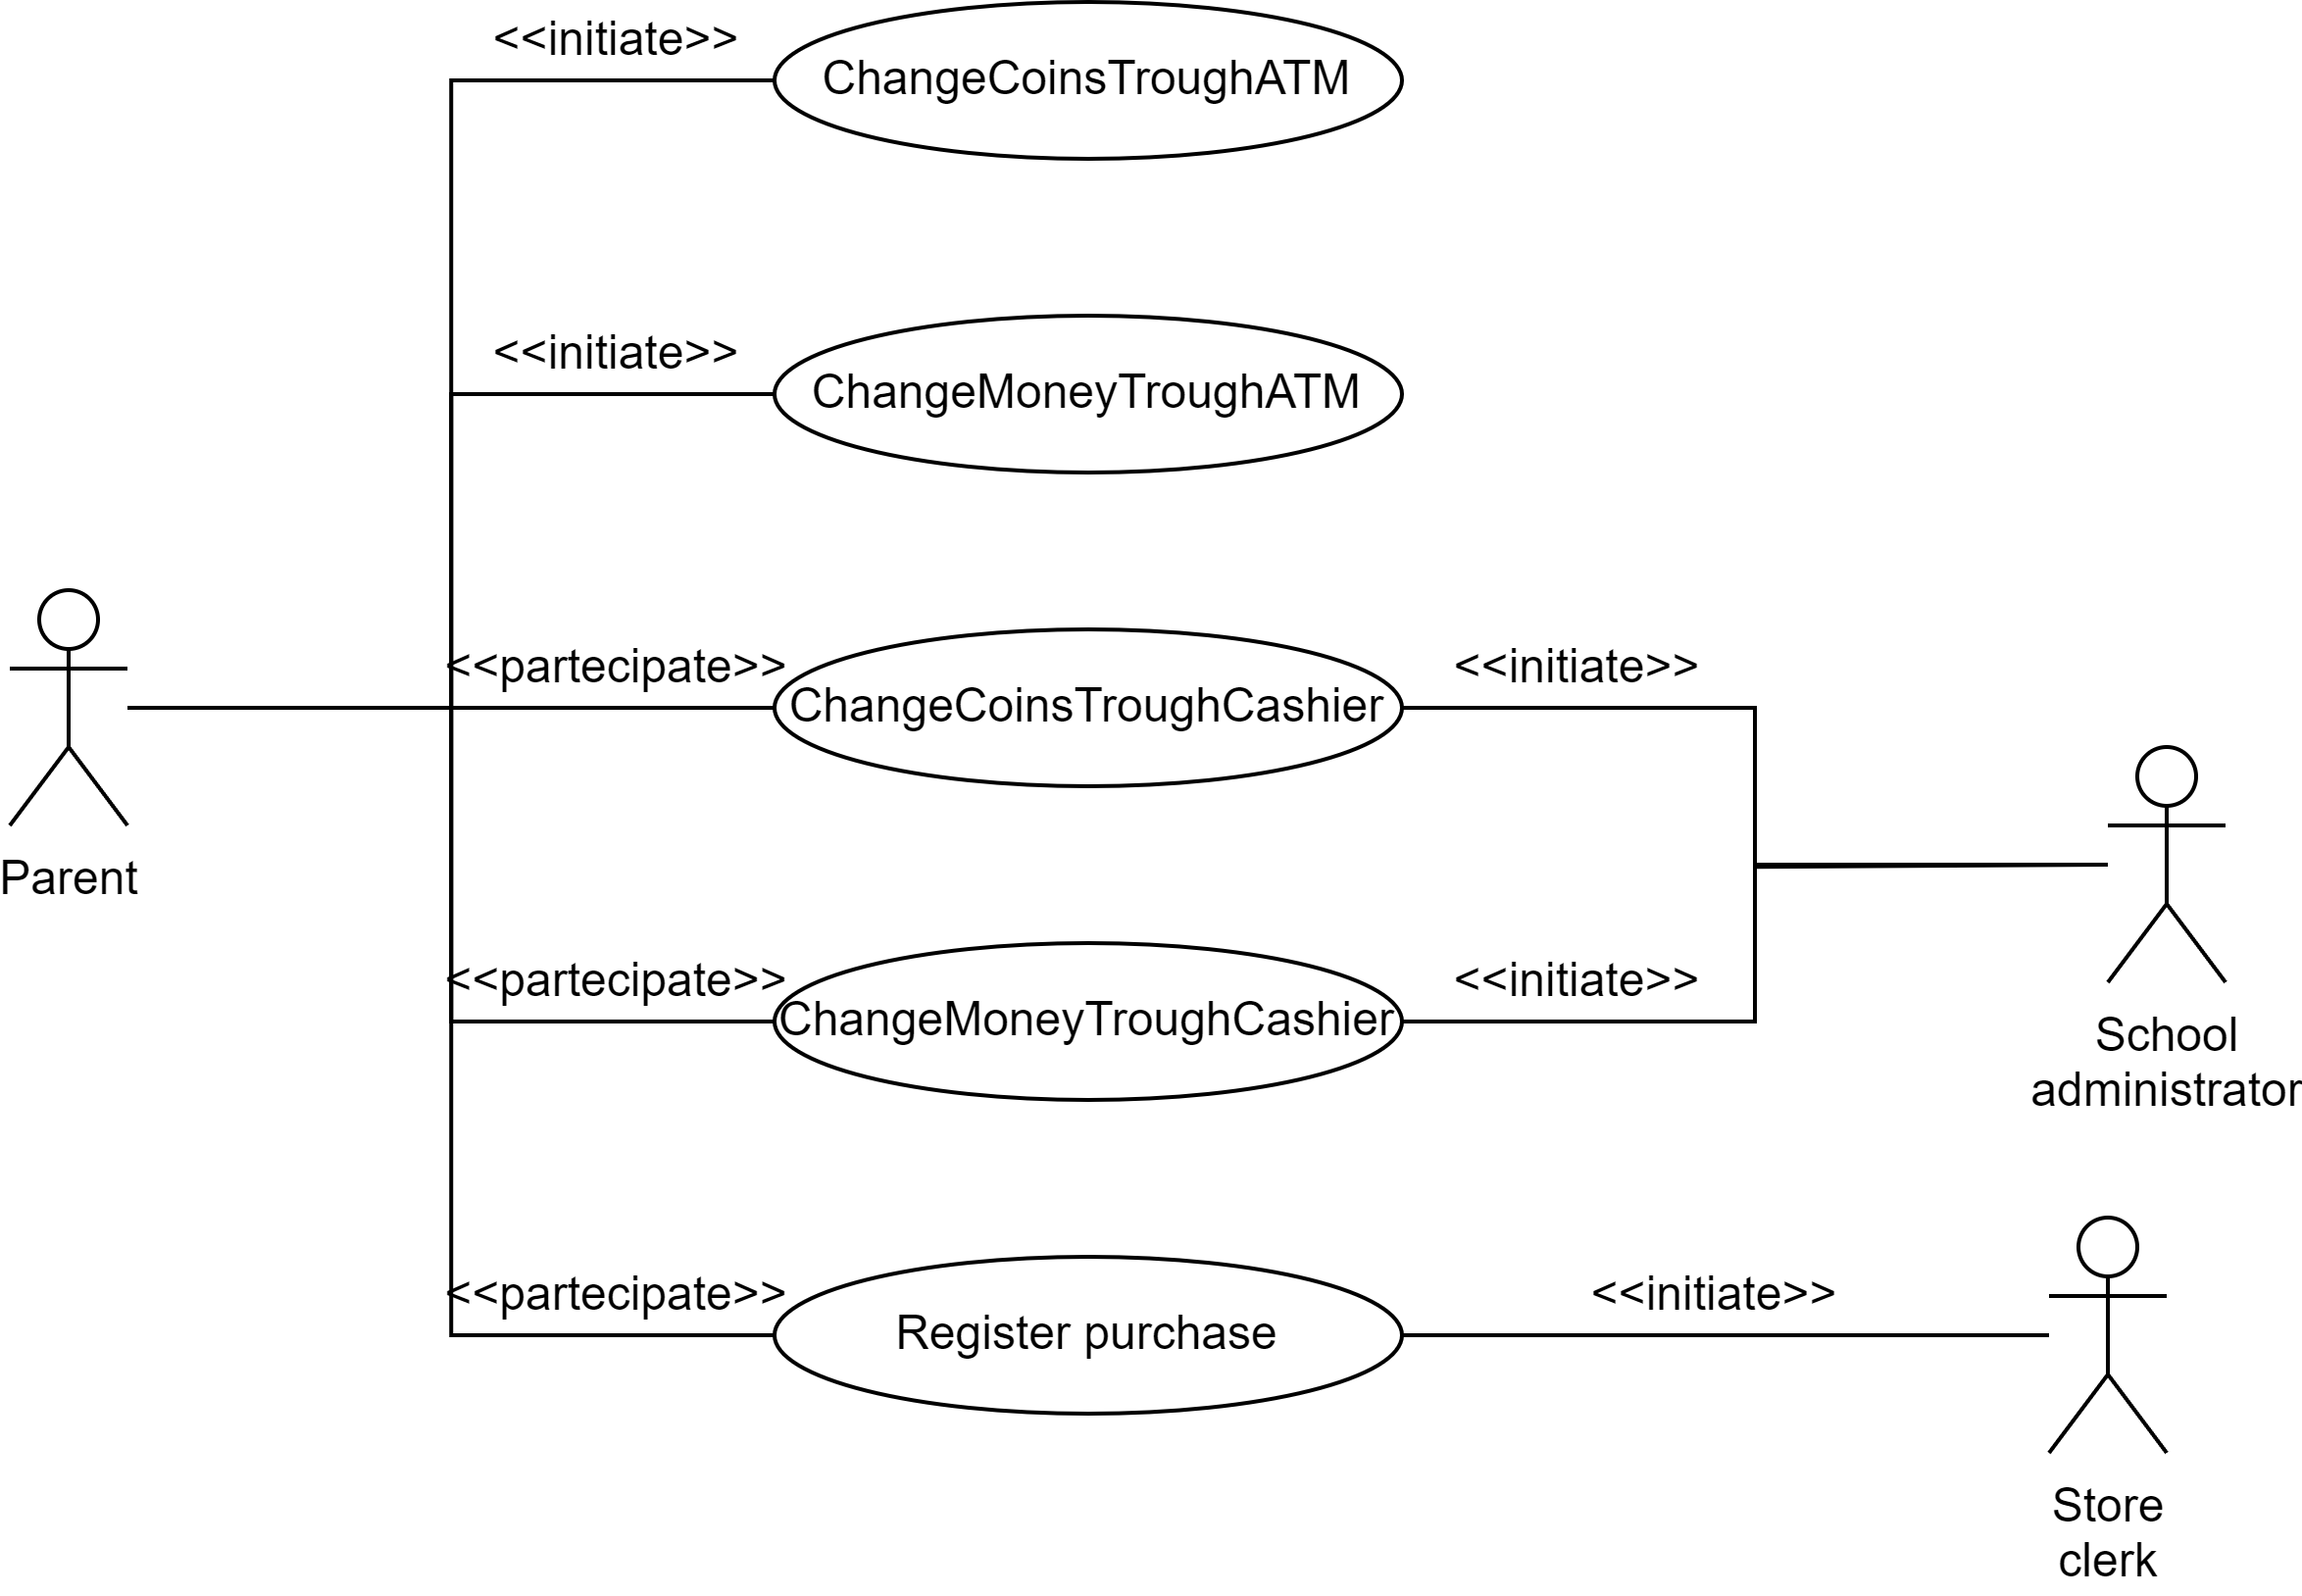
\includegraphics[width=0.9\linewidth]{images/usecase2.png}
                \end{figure}
        \end{enumerate}
    
    \newpage

    \chapter{Exercise session II}
    \section{Alloy}
        Consider construction cubes of three different sizes, small, medium, and large. You can build towers by piling up these cubes one on top of the other respecting the following rules:
        \begin{itemize}
            \item A large cube can be piled only on top of another large cube.
            \item A medium cube can be piled on top of a large or a medium cube.
            \item A small cube can be piled on top of any other cube.
            \item It is not possible to have two cubes, A and B, simultaneously positioned right on top of the same other cube C. 
        \end{itemize}
        \begin{enumerate}
            \item Model in Alloy the concept of cube and the piling constraints defined above.
            \item Model also the predicate canPileUp that, given two cubes, is true if the first can be piled on top of the second and false otherwise.
            \item Consider now the possibility of finishing towers with a top component having a shape that prevents further piling, for instance, a pyramidal 
                or semispherical shape. This top component can only be the last one of a tower, in other words, it cannot have any other component piled on it.
                Rework your model to include also this component. You do not need to consider a specific shape for it, but only its property of not allowing further 
                piling on its top. Modify also the canPileUp predicate so that it can work both with cubes and top components.
        \end{enumerate}
    \subsection*{Solution}
    \begin{enumerate}
        \item The concept of cube and its constraints can be defined in the following way. 
            \begin{lstlisting}[language=alloy]
abstract sig Size{}

sig Large extends Size{} 

sig Medium extends Size{} 

sig Small extends Size{}

sig Cube {
    size: Size,
    piledOn: lone Cube
}{piledOn != this}

fact noCircularPiling {
    no c: Cube | c in c.^piledOn
}

fact pilingUpRules {
    all c1, c2: Cube | c1.piledOn = c2 implies (
    c2.size = Large or
    c2.size = Medium and (c1.size = Medium or c1.size = Small) or c2.size = Small and c1.size = Small)
}

fact noMultipleCubesOnTheSameCube {
    no disj c1, c2: Cube | c1.piledOn = c2.piledOn
}
            \end{lstlisting}
        \item The predicate canPileUp can be defined as follows. 
            \begin{lstlisting}[language=alloy]
pred canPileUp[cUp: Cube, cDown: Cube] {
    cUp.piledOn = cDown and
    (cDown.size = Large or
    cDown.size = Medium and (cUp.size = Medium or cUp.size = Small) or 2
    cDown.size = Small and cUp.size = Small) 
}

pred show {} 

run show

run canPileUp
            \end{lstlisting}
        \item The now model become: 
            \begin{lstlisting}[language=alloy]
abstract sig Size{}

sig Large extends Size{} 

sig Medium extends Size{} 

sig Small extends Size{}

abstract sig Block{ 
    piledOn: lone Cube
}

sig Cube extends Block { 
    size: Size
}{piledOn != this}

sig Top extends Block { }

fact noCircularPiling {
    no c: Cube | c in c.^piledOn
}

fact noMultipleBlocksOnTheSameCube {
    no disj b1, b2: Block | b1.piledOn = b2.piledOn
}

fact pilingUpRules {
    all c1, c2: Cube | c1.piledOn = c2 implies (
    c2.size = Large or
    c2.size = Medium and (c1.size = Medium or c1.size = Small) or c2.size = Small and c1.size = Small)
}

pred canPileUp[bUp: Block, cDown: Cube] {
    bUp.piledOn = cDown and (bUp in Top or
    (cDown.size = Large or
    cDown.size = Medium and (bUp.size = Medium or bUp.size = Small) or cDown.size = Small and bUp.size = Small))
}   

pred show {} 

run show

run canPileUp 
            \end{lstlisting}
    \end{enumerate}

    \section{Alloy}
        The company TravelSpaces decides to help tourists visiting a city in finding places that can keep their luggage 
        for some time. The company establishes agreements with small shops in various areas of the city and 
        acts as a mediator between these shops and the tourists that need to leave their luggage in a safe
        place. To this end, the company wants to build a system, called LuggageKeeper, that offers tourists 
        the possibility to: look for luggage keepers in a certain area; reserve a place for the luggage in 
        the selected place; pay for the service when they are at the luggage keeper; and, optionally, rate 
        the luggage keeper at the end of the service.
        
        Given the scenario above, consider the following world phenomena:
        \begin{itemize}
            \item Every user owns various pieces of luggage.
            \item Every user can carry around various pieces of luggage.
            \item Each piece of luggage can be either safe, or unsafe.
            \item Small shops store the luggage in lockers, where each locker can store at most one piece of luggage. 
        \end{itemize}
        
        Consider also the following shared phenomena:
        \begin{itemize}
            \item Each locker is opened with an electronic key that is associated with it (the electronic key is regenerated at each use of the locker; also, a locker that does not have an electronic key associated with it is free).
            \item Each user can hold various electronic keys. 
        \end{itemize}

        Formalize through an Alloy model:
        \begin{enumerate}
            \item The world and machine phenomena identified above.
            \item A predicate capturing the domain assumption D1 that a piece of luggage is safe if, and only if, it is with its owner, or it is stored in a locker that has an associated key, and the owner of the piece of luggage holds the key of the locker.
            \item A predicate capturing the requirement R1 that a key opens only one locker.
            \item A predicate capturing the goal G1 that for each user all his/her luggage is safe.
            \item A predicate capturing the operation GenKey that, given a locker that is free, associates with it a new electronic key.
        \end{enumerate}
    \subsection*{Solution}
        The model requested is: 
        \begin{lstlisting}[language=alloy]
abstract sig Status{}

one sig Safe extends Status{} 

one sig Unsafe extends Status{}

sig Luggage{
    luggageStatus : one Status
}

sig EKey{}

sig User{
    owns : set Luggage, carries : set Luggage, hasKeys : set EKey
}

sig Locker{
    hasKey : lone EKey, storesLuggage : lone Luggage
}

sig Shop{
    lockers : some Locker
}

pred D1 {
    all lg : Luggage | lg.luggageStatus in Safe 
    iff 
    all u : User | lg in u.owns implies ( lg in u.carries or some lk : Locker | lg in lk.storesLuggage and lk.hasKey != none and lk.hasKey in u.hasKeys )
}

pred R1 {
    all ek : EKey | no disj lk1, lk2: Locker | ek in lk1.hasKey and ek in lk2.hasKey
}

pred G1 {
    all u : User | all lg : Luggage | lg in u.owns implies lg.luggageStatus in Safe
}

pred GenKey[lk, lk' : Locker] {
    lk.hasKey = none
    lk'.storesLuggage = lk.storesLuggage
    one ek : EKey | lk'.hasKey = ek 
}
        \end{lstlisting}
\end{document}